%----------------------------------------------------------------------------
\chapter{Gráfadatbázisok}
%----------------------------------------------------------------------------

Ez a fejezet az adatbázisrendszerek egy típusáról, a gráfadatbázisokról szól. Egy egyszerű példán keresztül megmutatjuk, hogy adott esetben miért lehet gyorsabb és ezáltal jobb a relációs adatbázisrendszereknél.

\section{Definíció}

Gráfadatbázisnak nevezünk minden olyan adatbázist, ahol az adat és/vagy a séma gráffal van reprezentálva, és minden adatmanipuláció egy gráftranszformációnak feleltethető meg.\cite{angles2008survey} Sokféle implementáció terjedt el, ami illeszkedik erre a definícióra. Különbséget tehetünk az alapján hogy a csúcsokban csak egyedeket tárolunk vagy a csúcsok csak azonosítók és az éleken keresztül a leveleken vannak a tulajdonságaik. Másik megközelítés, hogy az éleknek lehetnek-e tulajdonságaik vagy nem, illetve irányított vagy nem irányított a kapcsolat. 

A struktúrájából adódóan olyan adatok leírására alkalmasak leginkább, ahol az egyedek közötti kapcsolat számottevő.\cite{Neo4JGraphDatabase} Az éleken keresztül könnyen lehet navigálni, ezért alkalmasak közösségi hálózatok, keresőmotorok implementálására. 

\section{Példa gráfadatbázis használatára}

A gráfadatbázisok bemutatására a legáltalánosabb a közösségi hálózatok példája. Ennek alapja, hogy személyekről tárolunk bizonyos információkat, továbbá tároljuk a közöttük lévő kapcsolatokat. Esetünkben ez a kapcsolat legyen egyfajta és jelentse azt, hogy két ember ismeri egymást (barátok). Tároljuk a személyekről a következő adatokat:
\begin{itemize}
	\item Név
	\item Személyiigazolvány-szám
	\item További barátok listája
\end{itemize} 
Ezt egy relációs adatbázisban nehezen tudjuk megtenni, ugyanis a barátok listáját egy tömbben vagy lista típusban lenne célszerű tárolni, azonban a legtöbb relációsadatbázis-kezelő ezt nem támogatja. Általában egy második tábla felvételével szokták ezt megoldani. Ez a második tábla csak a kapcsolatok leírását szolgálja.

\begin{figure}[H]
	\centering
	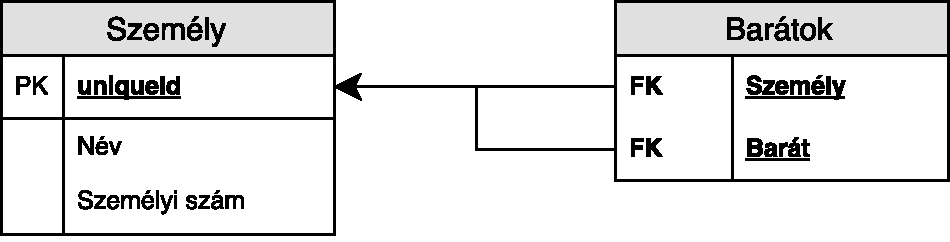
\includegraphics[width=100mm]{figures/RelaciosPelda.pdf}
	\caption{Példa relációs táblával való leírásra.}
	\label{fig:relaciosPelda}
\end{figure}

Amennyiben egy személy barátainak nevét szeretnénk megkapni, akkor ennek a relációs kalkulussal való kifejezése a következőképpen írható le:

\begin{equation}
\begin{split}
\{t^{(3)}\ | Szem\acute{e}ly(t) \wedge{} (\exists{}u^{(2)})Bar\acute{a}tok(u) \wedge{} (\exists{}v^{(3)})Szem\acute{e}ly(v) \wedge{} \\ v[1] = \textquoteright{}uniqueid\textquoteright{} \wedge{} 
t[1]=u[2] \wedge{}u[1]=v[1]      \}
\end{split}
\end{equation}

Már egy ilyen egyszerű kérdés megválaszolásához is három táblát kell összekapcsolni. Ez hatalmas erőforrást igényel, nem is beszélve arról, hogy mi a helyzet akkor, ha tranzitív lezártat szeretnénk számolni a baráti kapcsolat mentén. Ilyen esetben sokkal célravezetőbb az, ha egy gráfadatbázisban tároljuk az elemeket. A baráti kapcsolat általában kétirányú dolog, így a példánkban irányítatlan gráfon ábrázoljuk a kapcsolatot, de irányított gráffal is lehetne, ez esetben minden él helyére két él kellene.

\begin{figure}[H]
	\centering
	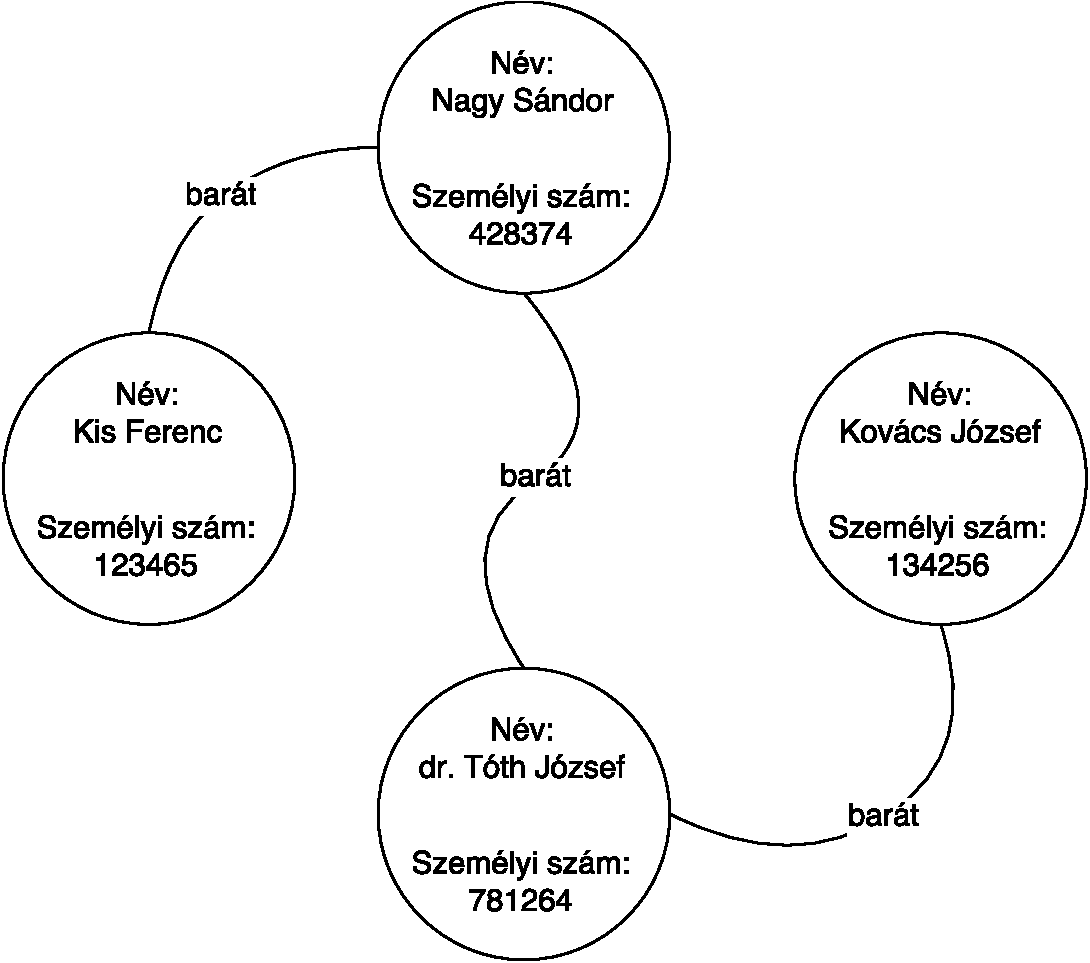
\includegraphics[width=100mm]{figures/GrafadatbazisPelda.pdf}
	\caption{Példa gráfadatbázisban való tárolásra.}
	\label{fig:grafPelda}
\end{figure}

A \ref{fig:grafPelda}. ábrán látható, hogy amennyiben valakinek barátait szeretnénk megtudni, a gráf élén végighaladva csak és kizárólag a barátainak az adatait fogjuk lekérni, senki másét nem. Ezáltal rengeteg memóriát és számolási időt takaríthatunk meg.